\section{Amélioration des performances}
\author{Kévin Moreau}


\begin{frame}
	\frametitle{Objectifs}

	\begin{block}{Les tâches à effectuer}
	 \begin{itemize}
      \item Amélioration de la plateforme Aerogear ;
	  \item Création d'un outil de lancement de l'environnement complet de Dynamease;
	  \item Mise en place des outils de mesure de performance;
	  \item Amélioration des applications Téléphoniques.
	 \end{itemize}
	\end{block}

	\begin{block}{Amélioration des Applications téléphoniques}
		\begin{itemize}
			\item Récupération rapide des contacts téléphoniques;
			\item Recherche rapide et pertinente sur la liste de contact;
			\item Récupération des images de profil des contacts Dynamease.
		\end{itemize}
	\end{block}

    
\end{frame}

\begin{frame}
	\frametitle{Mise en place de l'outil (1/5) : Cahier des charges}

    \begin{block}{Cahier des charges}
	 \begin{itemize}
	  \item Permettre le démarrage d'un environnement Dynamease;
	  \item Utiliser des bases de données pré-remplies;
	  \item Être utilisé facilement par les employés et consultants de Dynamease;
	 \end{itemize}
	\end{block}

\end{frame}

\begin{frame}
	\frametitle{Mise en place de l'outil (2/5) : Docker}

    \begin{block}{Présentation}
	 \begin{itemize}
	  \item Logiciel OpenSource;
      \item Automatisation du déploiement d’applications;
	  \item Utilise le Kernel de la machine sous-jacente.
	 \end{itemize}
	\end{block}

	\begin{block}{Termes importants}
	 \begin{description}
	  \item [Image] Configuration d’une application au sein d'un environnement Docker
	  \item [Container] L'exécution d'une image Docker
	  \item [Volume] Répertoire partagé entre le container et la machine sous-jacente
	  \item [Link] Un lien entre deux containers
	 \end{description}
	\end{block}

\end{frame}

\begin{frame}
	\frametitle{Mise en place de l'outil (3/5) : Les données}

    \begin{block}{Les types de données}
		\begin{itemize}
			\item Données de configuration du serveur;
			\item Données de stockage d'informations .
		\end{itemize}
	\end{block}

	\begin{block}{Solution pour l'intégration de ces données}
		\begin{enumerate}
			\item Utiliser les volumes;
			\item Utiliser un container de données .
		\end{enumerate}
	\end{block}


\end{frame}

\begin{frame}
	\frametitle{Mise en place de l'outil (4/5) : Ordre de lancement}

    \begin{center}
	  \begin{figure}
        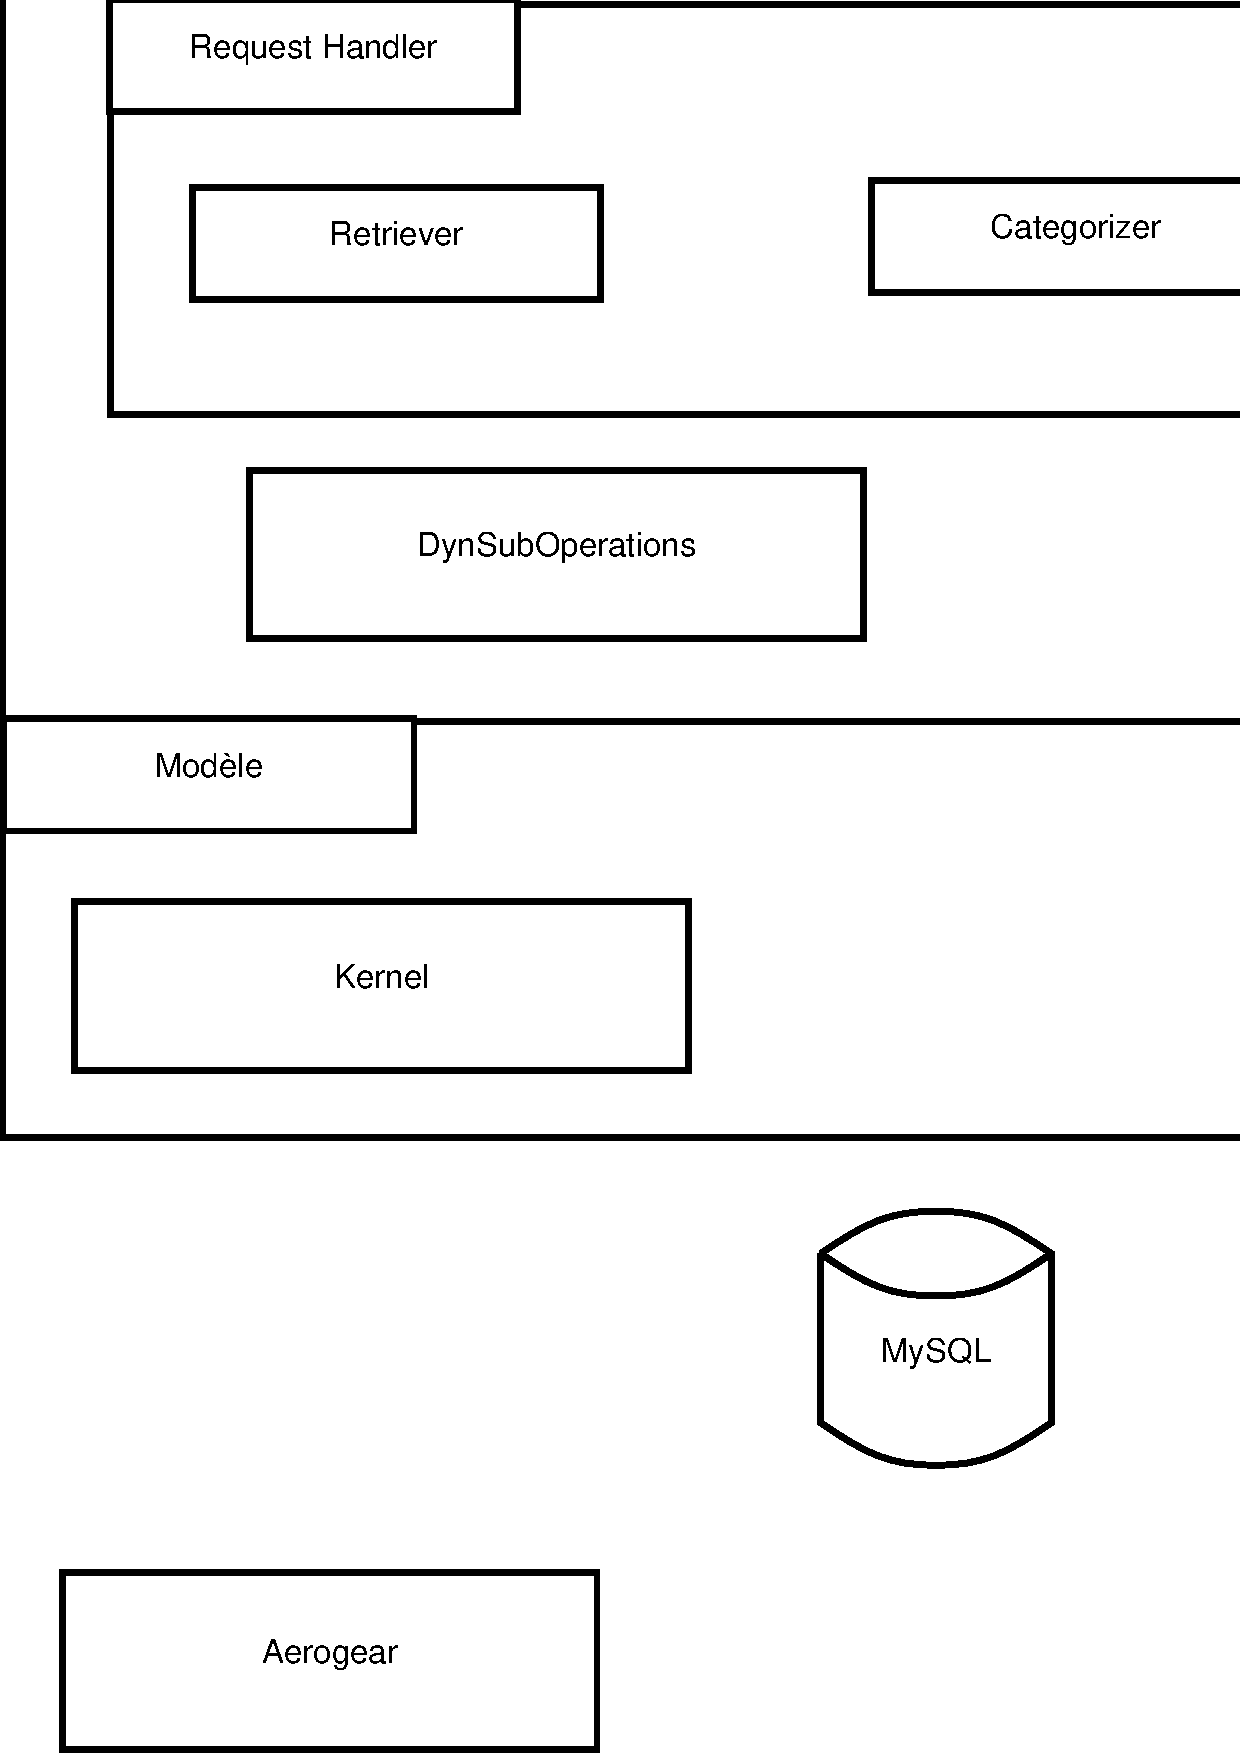
\includegraphics[scale=0.20]{images/pyramide.pdf}
	   \caption{Ordre de lancement des services0}
	  \end{figure}
	\end{center}
\end{frame}


\begin{frame}
	\frametitle{Mise en place de l'outil (5/5) : Fonctionnement}

    \begin{center}
	  \begin{figure}
        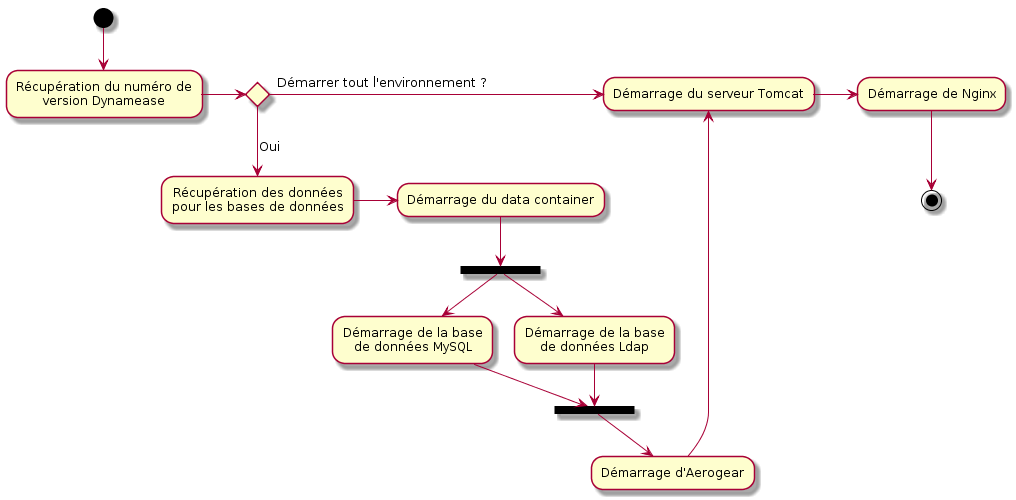
\includegraphics[scale=0.30]{images/activity_outil.png}
	   \caption{Diagramme d'activité du démarrage des services de Dynamease}
	  \end{figure}
	\end{center}

\end{frame}

\begin{frame}
	\frametitle{Amélioration de la recherche dans la liste de contact (1/3) : Explication}

    \begin{columns}[t]
  \begin{column}{5cm}
	  \begin{block}{Les étapes à suivre}
	    \begin{itemize}
	    	\item Étudier le code déjà existant;
	    	\item Détecter les anomalies et les sources d'amélioration;
	    	\item Recherche de solutions;
	    	\item Mise en place de la solution la plus pertinente.
	    \end{itemize}
	  \end{block} 
  \end{column}
  
  \begin{column}{5cm} 
  	\begin{center}
	  \begin{figure}
	   \caption{Liste de contact avec une recherche}
        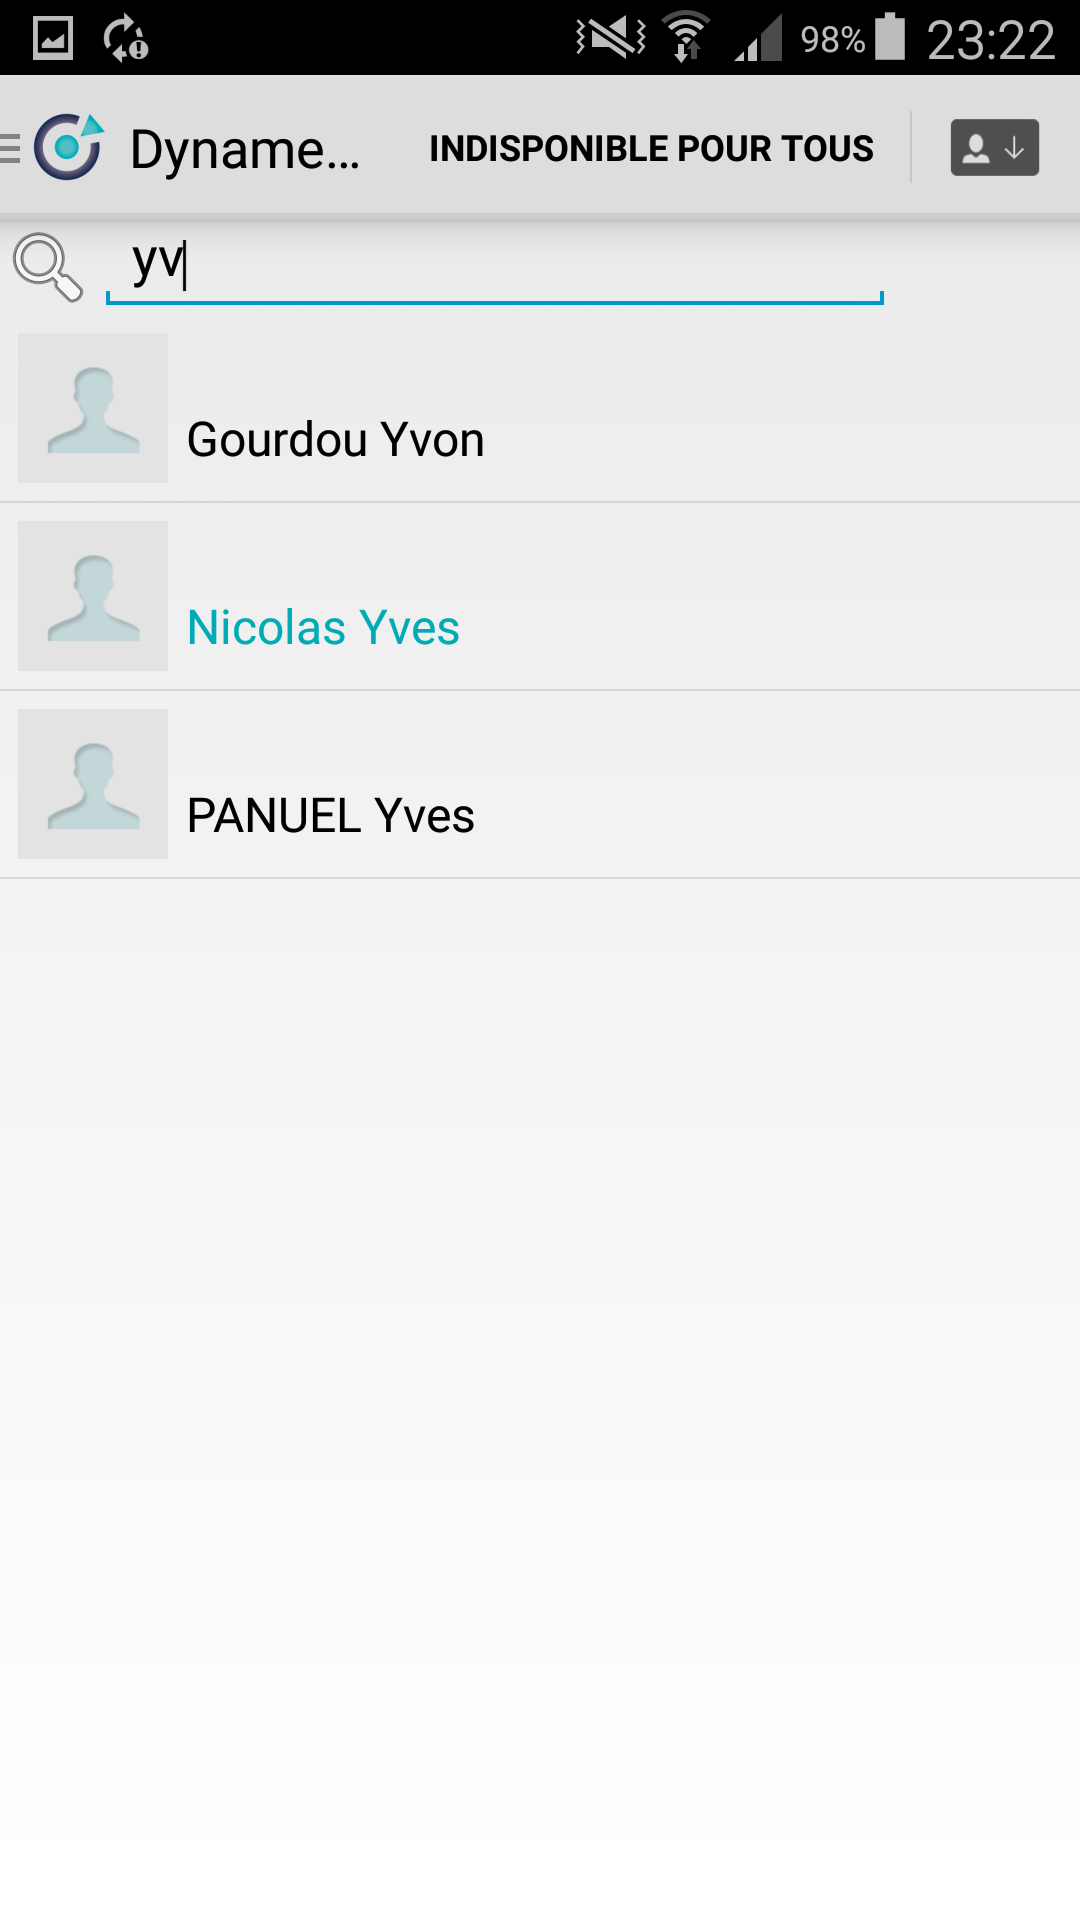
\includegraphics[scale=0.08]{images/recherche.png}
	  \end{figure}
	\end{center} 
  \end{column}
 \end{columns} 

\end{frame}

\begin{frame}
	\frametitle{Amélioration de la recherche dans la liste de contact (1/3) : Ancienne version}

    \begin{center}
	  \begin{figure}
        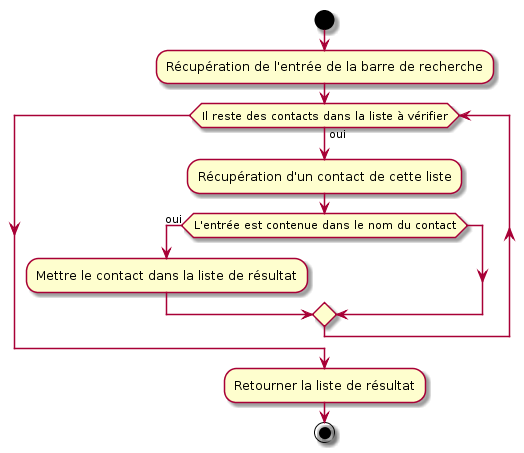
\includegraphics[scale=0.30]{images/activity_retrieve_old.png}
	   \caption{Diagramme d'activité de l'ancienne recherche}
	  \end{figure}
	\end{center}

\end{frame}

\begin{frame}
	\frametitle{Amélioration de la recherche dans la liste de contact (1/3) : Nouvelle version}

    \begin{center}
	  \begin{figure}
        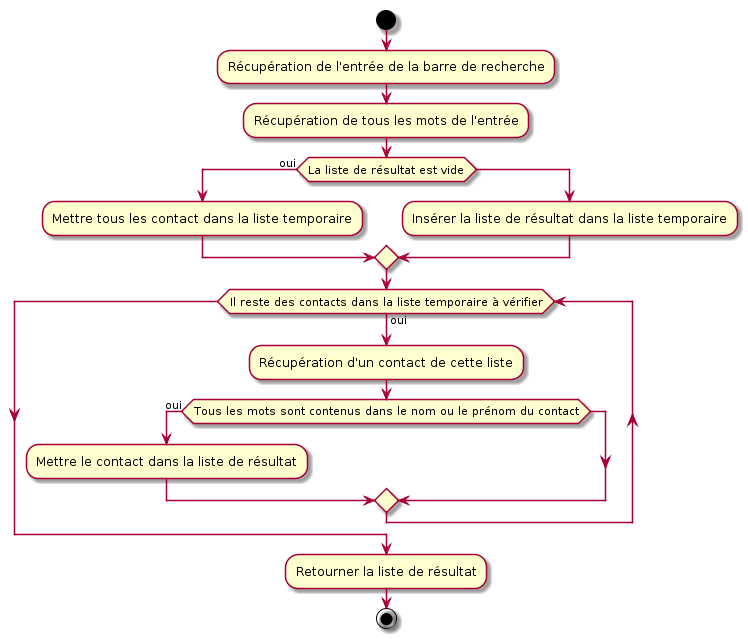
\includegraphics[scale=0.25]{images/activity_retrieve_better.png}
	   \caption{Diagramme d'activité de la nouvelle recherche}
	  \end{figure}
	\end{center}

\end{frame}